% Chapter 2
\documentclass[oneside, 12 pt]{book}
\usepackage{amsmath, amssymb}
\DeclareMathOperator*{\argmax}{argmax}

\usepackage[english]{babel}
\usepackage{microtype} %Tidyness
\usepackage{dsfont} %math 1
\usepackage[left = 4cm, right = 2.5cm, top = 2.5cm, bottom = 2.5cm]{geometry} %% Margin width
\linespread{1.5}
\usepackage{subfig} %% side by side figures
\usepackage{pdflscape} %%landscape pages
\usepackage{multirow} %% Multi Rows in tables
\usepackage{hyperref} %hyperlink table of contents
%\usepackage{algorithm}
%\usepackage{algorithmicx}
\usepackage{algpseudocode}
\usepackage{textcomp}
\usepackage{eurosym} %eurosymbol
\usepackage{graphicx}
\setcounter{secnumdepth}{4} %numbering for subsubsection 
\usepackage[Sonny]{fncychap} %Chapter Titles
\usepackage{afterpage} %spacing before landscape
\usepackage[version=3]{mhchem} % For Ca^2+
\let\oldemptyset\emptyset % empty set symbol
\usepackage{bbm} % for \mathbbm{}
\usepackage{bm}
\usepackage{mathtools} % for \splitdfrac{}

% Colours
\usepackage[dvipsnames]{xcolor}
\definecolor{col1}{RGB}{102, 194, 165}
\definecolor{col2}{RGB}{252, 141, 98}
\definecolor{col3}{RGB}{141, 160, 203}
\definecolor{col4}{RGB}{231, 138, 195}
\definecolor{col5}{RGB}{166, 216, 84}
\usepackage{colortbl} %colour table
% Algorithms 
%\usepackage{algorithm}
\usepackage[ruled,vlined]{algorithm2e}
%\usepackage[noend]{algpseudocode}
\makeatletter
\def\BState{\State\hskip-\ALG@thistlm}
\makeatother
%\usepackage[]{algorithm2e}

% Formatting for steps.
\usepackage{enumitem}
\newlist{steps}{enumerate}{1}
\setlist[steps, 1]{label = \it Step \arabic*:}

%Headers and Footers
\usepackage{fancyhdr}
\setlength{\headheight}{15pt}

\pagestyle{fancy}
\renewcommand{\chaptermark}[1]{ \markboth{#1}{} }
\renewcommand{\sectionmark}[1]{ \markright{#1} }

\fancyhf{}
\fancyhead[LE,RO]{\thepage}
\fancyhead[RE]{\ifnum \value{chapter}>0  Chapter \nouppercase{\thechapter : \leftmark} \fi} 
\fancyhead[LO]{ \ifnum \value{chapter}>0 Chapter \nouppercase{\thechapter : \leftmark} \fi } 

\fancypagestyle{plain}{ %
  \fancyhf{} % remove everything
  \renewcommand{\headrulewidth}{0pt} % remove lines as well
  \renewcommand{\footrulewidth}{0pt}
}
\AtBeginDocument{%
  \addtocontents{toc}{\protect\thispagestyle{empty}}%
  \addtocontents{lof}{\protect\thispagestyle{empty}}%
}
\graphicspath{{figures/}{../figures/}}
%\DeclareUnicodeCharacter{2212}{-}
 
\usepackage{blindtext}

%Add line numbers
 \usepackage{lineno}
\linenumbers

\begin{document}
\chapter{Non-trivial Model Properties}
The model we have created has been analysed with methods well-known in the field of statistics. However, using these methods to our model brings unique issues/decisions. In this chapter we will discuss these complications and explain the decisions we make going forward. 

%% ISI distribution section.   
\section{ISI Distribution}

% Intro of the importance of the ISI distribution. What it involves and what it can inform us on. Why we care.
In this section we discuss the importance of the inter-spike interval (ISI) distribution. In Chapter 2 we gave an example whereby we created a time-dependent ISI distribution by extending the one dimensional  Gamma$(\gamma, \gamma)$ distribution. The extension is performed by applying a time-rescaling method via the intensity function $x(t)$ which accounts for the time-dependence of \ce{Ca^2+} spiking. This approach can be used for all  probability distributions defined on $(0,\infty)$, such as an Inverse Gaussian or Weibull probability distributions. We will demonstrate that the choice of the original distribution is crucial to how well the model fits the \ce{Ca^2+} data. Furthermore, we will explain how to create a time-dependent ISI distribution from any probability distribution on $(0,\infty)$. Care is required in constructing these inhomogeneous ISI distributions to avoid non-identifiability issues. We will show how to circumvent this problem whilst also providing biological meaning to the intensity function used in creating these models. 

% Stationary case, showing that the problem reduces to finding the ISI distribution using the ISI times.
To begin, let us first consider the case of stationary \ce{Ca^2+} spikes --- spikes that depend only on the time since the last spike and not the time of the experiment. Hence if a \ce{Ca^2+} spike occurs at time $s$ then the probability that the next spike occurs at time $t>s$ only depends on the time between spikes $\tau = t-s$. Thus, we can convert a spike sequence $\{y_i\}^N_{i=1}$ into a sequence of ISIs $\{\tau_i\}^{M}_{i=1}$, where $\tau_i = y_{i+1} - y_{i}$ and $M = N-1$. Note that the time until the first spike  and the time from the last spike to the end of the experiment do not correspond to ISIs so we ignore them. Thus we can treat each $\tau_i$ as an observation of an unknown random variable $Y$ which describes the stationary ISI distribution. Since the ISI times can only take positive values the sample space of $Y$ is $(0,\infty)$. 

%Explain how apriori we have little knowledge of what shape the ISI follows.
Before we can use observed ISI times to estimate the ISI distribution we need to give structure to the ISI distribution. One method is to assume that $Y$ comes from a known family of probability distributions, such as the Exponential or Gamma distributions. However, it is not obvious which family of distributions will best describe the ISI dynamics. If we assume that $Y$ comes from, say the Exponential distribution, we call this the Exponential model for the ISI distribution.  Thus, we shall test several different models to find which describes the \ce{Ca^2+} ISIs the best. The models we consider are: the Exponential, Gamma, Weibull, Inverse Gaussian and Log Normal distributions. 

% Justify each of the distributions we use. 
 We consider the Exponential distribution because is the simplest distribution of $(0,\infty)$, and it acts as a useful base case to compare more complex ISI models. Moreover, the Exponential distribution is the only distribution on $(0,\infty)$ with the memoryless property \cite{ross98}. This means that if a spike occurs at time $s$ the probability of the next spike occurring at time $t$ is the same as the probability of the next spike occurring at time $t+r$ given that no spike occurs in $(s,r)$. Thus, including this model allows us to test whether the time since the last spike influences the probability of the next spike occurring.  
 %Moreover, we find in Chapter {\color{red}5} that the exponential is the only distribution that allows for the inclusion of the refractory period directly. 
 The Gamma distribution offers a natural extension to the Exponential distribution, since it contains the Exponential distribution as a special case. The Gamma distribution is an appealing candidate for the ISI distribution because it is a probability distribution for a combination of events occurring for the first time. Therefore, each event could be interpreted as a \ce{Ca^2+} puff, and each spike occurs the first time that $\alpha$ puffs occur \cite{Powell_2020}. 
   The Weibull distribution can also be viewed as an extension to the Exponential distribution. The Weibull distribution is often used to describe the ``time to failure'' of some component where the failure rate is proportional to a power of time \cite{Weibull_2018}. For this reason, the Weibull distribution is justifiable if we believe \ce{Ca^2+} spikes depend on a power of time, i.e. if a spike is more likely to occur as time goes on. 
    Conceptually, \ce{Ca^2+} spikes have been described as first passage events \cite{Thurley_2011}. Thus, since the Inverse Gaussian has been used to model first passage problems with Brownian motion \cite{Chhikara_1976} it appears as a suitable candidate.   
    Moreover, it has been shown that the ISI distribution of several neuronal systems under approximately stationary conditions are unimodal and right skewed \cite{Barbieri_2001}. This supports the Log Normal distribution since it is unimodal and right-skewed. Furthermore, this also gives support to the Gamma, Inverse Gaussian and Weibull distributions. 

%Give the PDFs for each of the models.
We now define each probability distribution, in terms of a general random variable $Z$.  
The random variable $Z$ is said to have an Exponential distribution with rate $\alpha >0$, shown as $Z \sim \text{Exponential}(\alpha)$, if its probability density function is given by
\begin{equation}\label{eq:origExp}
	f^\mathrm{ex}_Z (z ; \alpha ) = \alpha e^{-\alpha z}.
\end{equation}
$Z$ is said to have a Gamma distribution with shape $\alpha >0$ and rate $\beta >0$, shown as $Z \sim \text{Gamma}(\alpha,\beta)$, if its probability density function is given by 
\begin{equation}\label{eq:origGamma}
	 f^\mathrm{G}_Z(z; \alpha, \beta ) = \frac{\beta^\alpha z^{\alpha-1} e^{-\beta z}}{\Gamma(\alpha)},
\end{equation}
where $\Gamma(\alpha)$ is the gamma function $\Gamma(\alpha) = \int^\infty_0 x^{\alpha-1}e^{-x}\mathrm{d}x$.
  $Z$ is said to have an Inverse Gaussian distribution with mean $\mu >0$ and shape $\lambda >0$, shown as $Z \sim \text{IG}(\mu,\lambda)$, if its probability density function is given by 
  \begin{equation}\label{eq:origIG}
  	f^\mathrm{IG}_Z(z; \mu, \lambda) =\sqrt{\frac{\lambda}{2 \pi z^3}} \exp \left\{- \frac{\lambda(z-\mu)^2}{2\mu^2 z} \right\}.
  \end{equation}
  $Z$ is said to have a Log Normal distribution with parameters $\mu \in (-\infty, \infty)$ and $\sigma^2 >0$, shown as $Z \sim \text{Lognormal}(\mu,\sigma^2)$, if its probability density function is given by 
  \begin{equation}\label{eq:origLN}
  	f^\mathrm{LN}_Z(z; \mu, \sigma^2) = \frac{1}{z\sigma \sqrt{2\pi}} \exp \left\{- \frac{\left( z-\mu \right)^2}{2\sigma^2} \right\}.
  \end{equation}
   $Z$ is said to have a Weibull distribution with scale $\lambda >0$ and shape $k >0$, shown as $Z \sim \text{Weibull}(\lambda, k)$, if its probability density function is given by
   \begin{equation}\label{eq:origWei}
   	f^\mathrm{W}_Z(z ; \lambda, k ) = \frac{k}{\lambda}\left( \frac{z}{\lambda}\right)^{k-1} e^{-\left( z/\lambda\right)^k}.
   \end{equation} 
 



% Small section on does this choice of distribution matter. 

% How to fit stationary model.
Now that we have defined our models for the ISI distribution we want to fit them to observed ISIs and also find which model describes the ISI distribution best. Suppose $Y$ comes from the family of probability distributions parameterised by the set $\theta$ with probability distribution given by $f(z|\theta)$. To fit the model we need to estimate the value of $\theta$ that best describes the ISI times $\boldsymbol \tau = \{\tau_i\}^{M}_{i=1}$. One such method is maximum likelihood estimation (MLE). This involves maximising the likelihood function such that under the assumed model the ISI times are most probable. The likelihood function $L(\theta)$ is the joint probability density of observing all the ISI times.  Since we are considering stationary \ce{Ca^2+} spikes, the joint probability function reduces to the product of the probabilities of individual ISI times giving
$$
L(\theta) = p(\tau_1,\tau_2, \dots, \tau_{M}| \theta) = \prod^{M}_{i=1} f(\tau_i|\theta).
$$
The maximal likelihood estimate $\hat \theta$ is the value of $\theta$ that maximises the likelihood
$$
\hat \theta  =  \argmax\limits_{\theta \in \Theta}  \left\{ \prod ^M_{i=1} f(\tau_i | \theta ) \right\},
$$
where $\Theta$ is the space of all possible parameter values. In the case of the Expo nential, Inverse Gaussian and Log Normal analytical solutions for the MLE exist. Namely, with observed ISI times $\boldsymbol \tau$, the MLE when $Y \sim \text{Exp}(\alpha)$ is $\hat \alpha = M/\sum^{M}_{i=1}\tau_i$, the inverse of the sample mean. If $Y \sim \text{IG}(\mu,\lambda)$ the MLE occurs at
 $$
 \hat \mu = \frac{1}{M}\sum^{M}_{i=1} \tau_i \qquad \text{and} \qquad  
 \frac{1}{\hat \lambda} = \frac{1}{M}\sum^{M}_{i=1}\left(\frac{1}{\tau_i} - \frac{1}{\hat \mu}\right).
 $$
  Finally, if $Y \sim \text{Lognormal}(\mu, \sigma^2)$ the MLE occurs at 
  $$\hat \mu = \frac{1}{M}\sum^{M}_{i=1}\log \tau_i  \qquad \text{and} \qquad \hat \sigma^2 = \frac{1}{M}\sum^{M}_{i=1}\left( \log \tau_i -\hat \mu \right)^2 $$

 However, a closed form solution of the MLE does not exist for either the Gamma nor Weibull distributions and thus numerical methods are required to calculate the MLE. We use the \texttt{optim} function from the \texttt{stats} package in the language R.  

%Bit on evaluating which is the best model. 

% Example using Ca data.
To visualise the difference between the five stationary ISI distribution models we fit each model to the same spike sequence generated by a HEK293 cell challenged with $10\mu \mathrm{M}$ Carbachol. The cell exhibited 66 \ce{Ca^2+} spikes and we convert the spikes into a sequence of ISI times --- shown as the black ticks on the x-axis of Figure \ref{fig:ExampleISI}. Subsequently, we calculate the MLE for each of the distributions. The results are shown in the second column of Table \ref{table:Stationary}. We compare the models by examining the log likelihood at the MLE, shown as the third column in Table \ref{table:Stationary}. The log likelihood will give an indication into which models perform better, where superior models will have a higher log likelihood than other models. The method is used as a simple tool to illustrate the fact that some models better suit the \ce{Ca^2+} spike data. Other more powerful tests could be done to compare the different models such as the Kolmogorov-Smirnov test \cite{Massey_1951} or Anderson-Darling test \cite{Anderson_1954}. We find that the Exponential is the worst model having a log likelihood significantly lower than the other models. The Inverse Gaussian model has the largest log likelihood, implying it fits the spike sequence the best. However, the log likelihood of the Gamma is similar, thus either model could be used to describe the spike sequence.

% Table of fitting stationary distributions.
\afterpage{%
\clearpage
\begin{table}[t!]
  \begin{center}
    \begin{tabular}{|l|l|l|}
    \hline
     Distribution & MLE of ISI parameter/s & Log Likelihood  \\ \hline
     \cellcolor{col1} Exponential & $\alpha = 0.0221 $ & $-312.75$ \\ 
    \cellcolor{col2} Gamma & $(\alpha, \beta) = (0.229,10.35)$ & $-261.86$ \\
     \cellcolor{col4} Inverse Gaussian & $(\lambda,\mu) = ( 442.13, 45.22)$ & $-261.06$ \\
     \cellcolor{col5} Log Normal & $(\mu, \sigma) = (3.762,0.312)$ & $-268.78$ \\
     \cellcolor{col3} Weibull & $(k, \lambda) = (3.226, 50.41)$ & $-266.48$\\ \hline
    \end{tabular}
    \caption{The MLE and log likelihood of the MLE of each distribution fit to \ce{Ca^2+} ISIs from a HEK293 cell challenged with $10\mu \mathrm{M}$ Carbachol. The colour of the distribution matches the colour of the probability densities shown in Figure \ref{fig:ExampleISI}. }
    \label{table:Stationary}
  \end{center}
\end{table} 

 \begin{figure}[h!]
   \begin{center} 
    \subfloat{{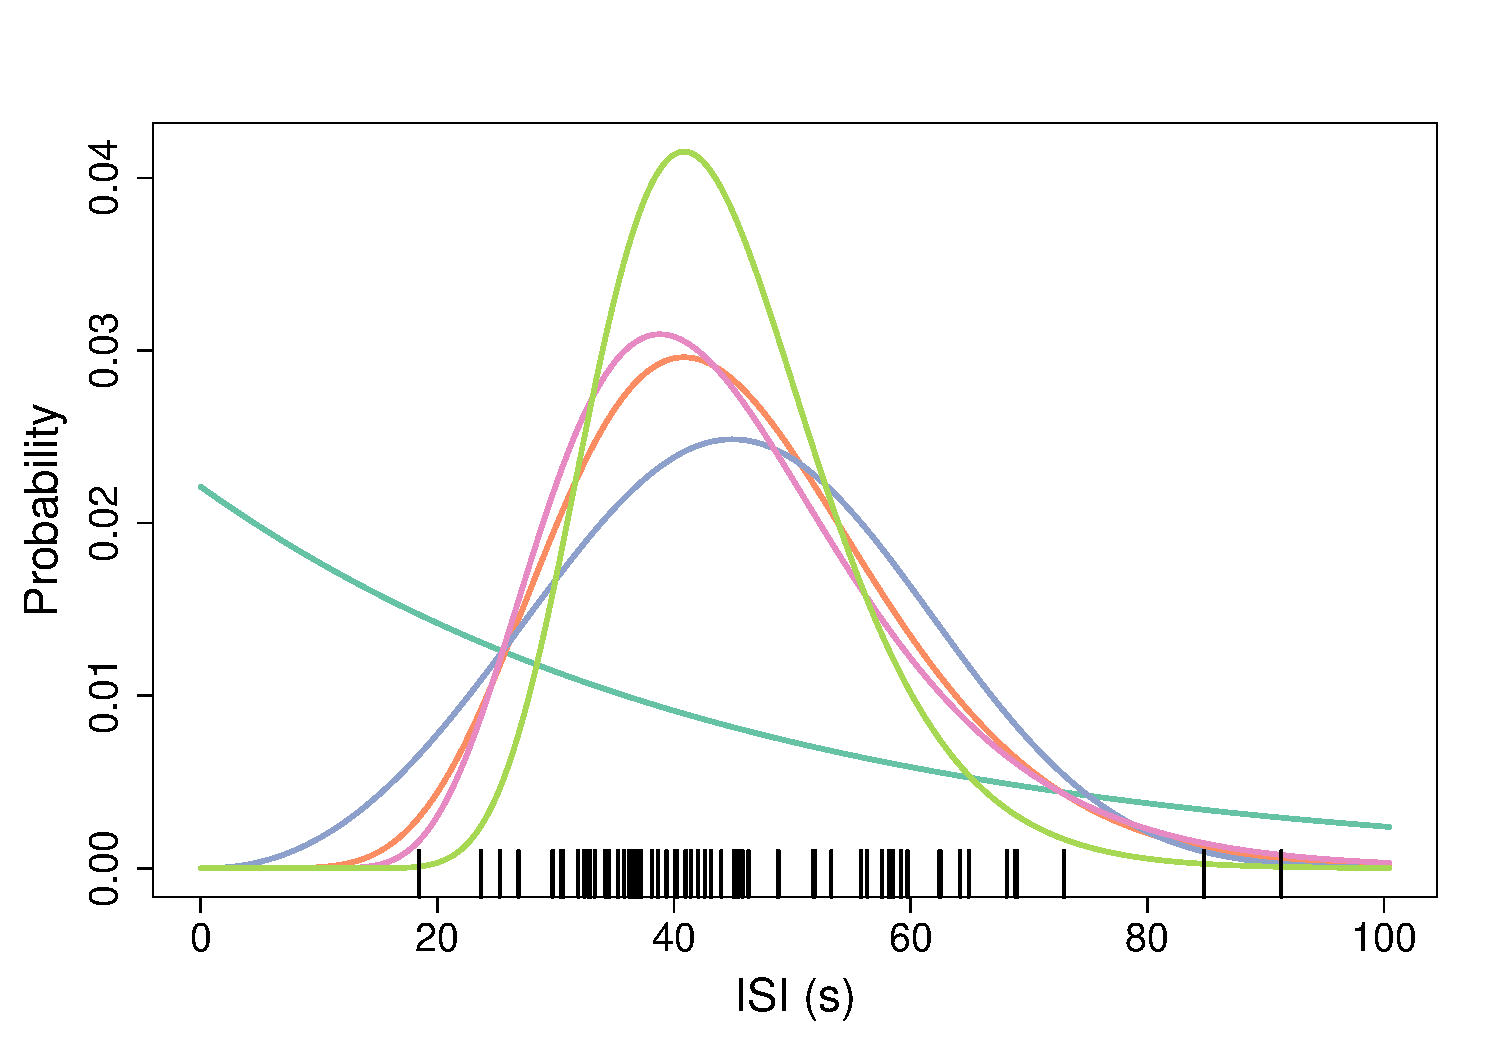
\includegraphics[width=0.8 \linewidth]{ISI_Stationary_plot} }}
    \end{center}     
    \caption{Probability density functions corresponding to the MLE of: an Exponential (dark green), a Gamma (orange), Inverse Gaussian (pink), Log Normal (light green) or Weibull Distribution (blue) fit to ISIs --- shown as black ticks on the x-axis.      }
    \label{fig:ExampleISI}
    \end{figure}
    \clearpage
}


 To explain this difference in performance we plot the probability density function  of the MLE for each model. This is shown in Figure \ref{fig:ExampleISI} where dark green, orange, pink, light green and blue correspond to the Exponential, Gamma, Inverse Gaussian, Log Normal and Weibull distributions respectively. We see that the largest proportion of spike times are centered around 40s, which is mirrored by the probability densities of all the distributions bar the Exponential. The Exponential model does not capture this due to the limitations of its shape, i.e. the mode of the exponential is zero. We see that the Gamma and Inverse Gaussian have similar probability density functions --- the pink and orange lines --- and hence similar likelihoods. We also find that the Log Normal and Weibull have similar central regions of the distribution as the Gamma and Inverse Gaussian but with narrower and wider tails respectively. Zooming in on the region between 0s and 20s we see a single ISI just before 20s. In this region we observe that the Weibull's probability density is too high --- we would expect more ISIs lower than 20s --- and the Log Normal's probability density is too low --- the density at the lowest ISI time is almost zero. This illustrates why the Log Normal and Weibull do not fit the ISIs as well as the Gamma and Inverse Gaussian models. 


%Summary of the stationary case. 
The above example demonstrates that the choice of ISI distribution is crucial, since we found that some distributions fit the \ce{Ca^2+} ISIs better than other distributions. This is due to the fact that the shape of the probability density function varies for each family of probability distributions. Thus, when considering the ISI distribution for non-stationary spike sequences we need to consider several distributions as some may  describe the \ce{Ca^2+} spikes better than others.

At this stage, one could argue to use a non-parametric method to estimate the ISI distribution, such as using splines or a Gaussian Process prior. This would indeed be a more flexible framework since the ISI distribution would not be limited to the shape of the chosen probability model. However, we have chosen to show this approach as our model for time-dependent \ce{Ca^2+} spikes generalises these ISI distributions. If we began by using a non-parametric method to model the stationary spike sequences it would be unclear how to generalise to a time-dependent model. For example, as each ISI does not necessarily have the same statistics, it is not possible to find a `common' ISI distribution that describes all ISIs. One way to visualise this is that in the stationary setting the `true' ISI distribution is a fixed function, whereas generalising to time-dependent spikes the ISI distribution varies as the experiment progresses.  



% WE ARE HERE
\hfill

%The IP distribution often serves as starting point for analysing spiking behaviour as it is the most basic statistical distribution. While the parsimony of the IP distribu- tion has undoubtedly helped in establishing a large body of mathematical results, real world data often exhibit more complex statistics. The IG distribution provides a natural extension of the IP distribution, in that it contains the IP distribution as a special case: putting γ = 1 in (5) recovers (10). The shape parameter γ endows the IG distribution with more flexibility, which has proven fruitful in numerous applications. Conceptually, spikes in general and Ca2+ spikes in particular have been described as first passage events [38]. One of the most fundamental models, which contains positive drift and random motion only, gives rise to the IIG distribution.




% TIME-DEPENDENT MODEL.
%Back to our model.
Now that we have shown the importance of the ISI distribution in the stationary case we want to generalise each distribution to allow for time-dependence. We consider the approach of Barbieri et al \cite{Barbieri_2001} which uses a time rescaling transformation. This approach was also utilised by Tilunaite et al \cite{AGNE:1} to model \ce{Ca^2+} spikes. However, both only apply the method to one-parameter versions of the Gamma and Inverse Gaussian distributions. In particular, they generalise a $\mathrm{Gamma}(\gamma, \gamma)$ for $\gamma > 0$ and an $\mathrm{IG}(\mu, 1)$ where $\mu > 0$. It is unclear why these particular one-parameter versions of the Gamma and Inverse Gaussian are taken as the initial stationary distribution. For example rather than rescaling $\mathrm{IG}(\mu, 1)$ where $\mu > 0$ another option could be to rescale $\mathrm{IG}(1, \lambda)$ where $\lambda >0$. Moreover, it is not obvious why you cannot time rescale the full Inverse Gaussian $\mathrm{IG}(\mu, \lambda)$.

% First the exponential distribution.
% Let us begin with the Exponential distribution. This differs from the other considered distributions because it only has a single parameter $\alpha$. A point process with identical Exponential$(\alpha)$ ISI distributions is known as a Poisson process with rate $\alpha$ because the  number of events in the interval $[s,t]$ is a Poisson random variable with mean $\alpha (t-s)$. The non-stationary generalisation of the Poisson process is called an inhomogeneous Poisson process, where the parameter $\alpha$ is replaced with a rate function $\alpha(t)$. Thus, we shall call the inhomogeneous  Exponential ISI distribution
%$$ p(t,s|\alpha) = \alpha(t) \exp \left\{ -\int^t_s \alpha(u) du \right\}. $$

% intensity rescaling general.
We begin by deriving the time dependent ISI distribution from a general stationary ISI distribution. 
Recall that the random variable $Y$ with probability density function $f(z|\theta)$ describes the stationary ISI distribution, where $z$ represents a ISI time. Since we are now concerned with a time-dependent model of the ISI distribution we need to explicitly state which ISI we are modelling.  Consider the $k$th spike $y_k$ that occurs at time $s$. The probability density of the next spike occurring at time $t > s$ is $f(t-s|\theta)$, in other words we have $z = t-s$. Thus, the random variable $Y_s$ describing the stationary ISI distribution of the next spike occurring after $y_k$ has probability density function $f(z|\theta)$ on support $s < z <\infty$. To account for the time dependence we map the original time $(s,\infty)$ to a new time via the one-to-one differentiable transformation $v(z) = \int^z_s x(u) du$, where $x$ is a positive function that accounts for the time dependence of the ISI times. Therefore, by applying the change of variables formula we create a new random variable $W$ describing the time-dependent ISI distribution with pdf $g(t|x,\theta)$ and support $0<t<\infty$, where
\begin{align*}
	g(t|x,\theta) =&  \lvert v'(t) \lvert \times  f(v(t)|\theta) ,  \\
	 =& x(t) f(\int^t_s x(u) du | \theta), \\
	 =& x(t) f(X(s,t) | \theta),
\end{align*}
 where $X(s,t) = \int^t_s x(u)du$. Note that the above result holds true for any time $s$ of the spike $y_k$. Thus the probability density of the next spike occurring at time $t$ given the last spike occurred at time $s$ is given by
 \begin{equation} \label{eq:transformation}
g(t,s| x,\theta) = x(t)f(X(s,t)|\theta). 	
 \end{equation}

% Example using the Gamma distribution
We can now apply the transformation to the stationary ISI distributions defined in \eqref{eq:origExp} to \eqref{eq:origWei} to construct inhomogeneous versions of the Exponential, Gamma, Inverse Gaussian, Log Normal and Weibull distributions.. 
For example by substituting \eqref{eq:origGamma} into \eqref{eq:transformation} we construct the inhomogeneous Gamma, where the probability density that the next spike occurs at time $t$ given the previous spike occurred at time $s$ is given by
\begin{align}\label{eq:InhomoGam2}
	g_{\mathrm{GAM}}(t,s | x, \alpha, \beta) &= x(t) f_{\mathrm{GAM}}(X(s,t)|\alpha,\beta), \nonumber \\
	  &=   \frac{\beta x(t)}{\Gamma ( \alpha )} \big[ \beta X(s,t) \big]^{\alpha -1} \exp \left\{ - \beta X(s,t)  \right\}. 
\end{align} 
Thus, we see that the time-dependent version of the ISI distribution consists of introducing the intensity function $x$ as a new parameter and where the original ISI time --- $z = t-s$ in equations \eqref{eq:origExp} to \eqref{eq:origWei} --- is replaced with the integral of the intensity function between $t$ and $s$. The intensity describes the time-dependent nature of the \ce{Ca^2+} spiking, where the larger the intensity is over an interval the more spikes we expect in that interval.  We also get a factor of $x(t)$ in the time-dependent ISI distribution from the time transformation. 


%Transition to non-identifiability issue. 
At this stage, we have constructed a model for time-dependent \ce{Ca^2+} spikes and if given the type of ISI distribution --- Exponential, Gamma, etc --- along with their parameters and the intensity function over the whole experiment time, we can simulate spike sequences. This is done by using the inverse transform method --- see Chapter 2. 

Next, we explore if we can infer the model parameters --- the intensity function and ISI parameters --- given a spike sequence.  Let us begin by considering the inhomogeneous Gamma ISI distribution --- shown in \eqref{eq:InhomoGam2}. Notice in the probability density that $\beta$ is always multiplied by either $x(t)$ or $X(s,t)$. This could lead to difficulty disentangling the parameters $\beta$ and $x$, since they may be non-identifiable.

%Basic non-identifiability  case
To visualise this issue, imagine we want to estimate the area of a rectangle. Since we know the area of a rectangle is given by its base $b$ multiplied by its height $h$ we choose to model the area in terms of the product $bh$. However, suppose we are given sample areas $A_1, A_2, \dots, A_N$, and we want to infer our parameters $b$ and $h$. This is not possible because the area does not give us enough information about $b$ and $h$, i.e if $b=1$ and $h=4$ this gives the same area as $b=2$ and $h=2$, thus we cannot identify $b$ and $h$. This gives a picture of non-identifiability issues. Strictly speaking a model is non-identifiable if two unique parametisations lead to identical probability distributions. Conversely, a probability model is identifiable if we can learn the true parameter values if given an infinite set of observations.

%Description for the Gamma ISI distribution.
Indeed, we find that the inhomogeneous Gamma ISI distribution is non-identifiable. 
Consider two inhomogeneous Gamma distributions with parameters $(x,\alpha,\beta)$ and $(xa, \alpha, \beta/a)$ for some $a>0$, respectively. Rearranging the latter yields

 \begin{align*}
 g_{\mathrm{GAM}}(t,s|ax, \alpha, \beta/a) &=  \frac{(\beta/a) ax(t)}{\Gamma ( \alpha )} \big[ (\beta/a) \int^t_s a x(u) du \big]^{\alpha -1} \exp\left\{ - (\beta/a) \int^t_s a x(u) du  \right\}, \\
 &=  \frac{\beta x(t)}{\Gamma ( \alpha )} \big[ (\beta/a) a\int^{t}_{s}  x(u) du \big]^{\alpha -1} \exp \left\{ - (\beta/a) a\int^{t}_{s}  x(u) du  \right\}, \\
  &=  \frac{\beta x(t)}{\Gamma ( \alpha )} \big[ \beta X(s,t) \big]^{\alpha -1} \exp\left\{ - \beta X(s,t)  \right\},\\
  &= g_{\mathrm{GAM}}(t,s|x, \alpha, \beta).
 \end{align*}
Thus, we found two unique parametisations with identical probability distributions. Hence, the Gamma ISI distribution is non-identifiable. Furthermore, we find that all the other considered time-dependent ISI distributions are also non-identifiable. This is shown in Table \ref{table:Non-ident}, where each distribution is given a pair of unique parameters sets that give rise to identical distributions --- for proof these parameter sets lead to identical distributions see Appendix {\color{red} XX}. 

%Maybe some line about the intensity replacing one of the parameters from the original distribution. 

% Table of Non-identifability
\begin{table}[h!]
  \begin{center}
    \begin{tabular}{|l|l|l|}
    \hline
     Distribution & Base parameters & Identical to ..  \\ \hline
     Exponential & $(x,\alpha)$ & $(ax, \alpha/x)$ \\
     Gamma & $(x, \alpha, \beta)$ & $(a x, \alpha, \beta/a)$ \\
     Inverse Gaussian & $(x,\lambda,\mu)$ & $(a x, a\lambda, a \mu)$ \\
     Log Normal & $(x,\mu, \sigma)$ & $(a x, \mu + \log a, \sigma )$ \\
     Weibull & $(x, k, \lambda)$ & $(a x, k, a \lambda)$\\ \hline
    \end{tabular}
    \caption{Parameterisations of the inhomogeneous ISI distributions which lead to non-identifiability, where $a>0$ is a constant. }
    \label{table:Non-ident}
  \end{center}
\end{table} 


% Non identifiability. 
%We first need to check if each parameter in the ISI distribution is identifiable. This means that we can theoretically learn the true values of the parameters if given an infinite number of observations. Moreover, a model is non-identifiable if two distinct parameterisations lead to identical probability distributions. 
This explains the use of one-parameter versions of the Gamma and Inverse Gaussian used in \cite{Barbieri_2001, AGNE:1}, since restricting the stationary distributions to a single parameter alleviates the non-identifiability. To picture this, return to the rectangle problem discussed previously. Constraining the stationary ISI distribution is similar to adding, the restriction that the rectangle must be a square. Then the base and height are equal and lead to a unique area $A = b^2 = h^2$. However, it is still unclear how to constrain the stationary probability distributions to resolve the non-identifiability. For example, we could restrict the stationary Gamma distribution from two parameters $(\alpha, \beta)$ to one parameter $\gamma$ by setting $\alpha = \beta = \gamma $ or $\alpha =\gamma$ and $\beta =\gamma^2$. There are infinitely many possibilities for constraining the stationary ISI distribution.  Thus we want to find a consistent approach to restrict these distributions whilst giving meaning to the remaining parameters.  

Recall that Barbieri and Tilunaite generalised a $\mathrm{Gamma}(\gamma, \gamma)$ and an $\mathrm{IG}(\mu, 1)$. Thus, the constrained Gamma distribution has mean equal to $1$ and variance equal to $1/\gamma$, whereas the constrained Inverse Gaussian has mean equal to $\mu$ and variance equal to $\mu^3$. From considering the mean and variance there is no clear pattern for how they constrained the stationary ISI distribution. Consider the probability density functions for the inhomogeneous ISI distributions constructed from an $\mathrm{IG}(\mu, 1)$ and a $\mathrm{Gamma}(\gamma, \gamma)$
 \begin{equation} \label{eq:IGAgne}
 	  g_{\mathrm{IG^*}}(t,s| x,\mu) =  \frac{x(t)}{\sqrt{2\pi X(s,t)^3}} \exp  \left\{ -\frac{(X(s,t)-\mu)^2}{2 \mu^2 X(s,t)}\right\} 
 \end{equation}

 and
 \begin{equation}\label{eq:GamAgne}
 	 g_{\mathrm{GAM^*}}(t,s| x, \gamma) =  \frac{\gamma x(t)}{\Gamma ( \gamma )} \big[ \gamma X(s,t) \big]^{\gamma -1} \exp \left\{ - \gamma X(s,t)  \right\},
 \end{equation}
respectively. Bear in mind that the corresponding stationary ISI distribution should be contained in the time-dependent model as a special case. Indeed, if we take the intensity function to be a constant, the time-dependent case reduces to its stationary counterpart. This is because the time-variability comes from the variability in the intensity function. Therefore, we set $s=0$ and substitute $x(t) = a$ into \eqref{eq:IGAgne}  giving
\begin{align}\label{eq:IGfixedx}
	 g_{\mathrm{IG^*}}(t,s| a,\mu) =& \frac{a}{\sqrt{2 \pi (at)^3}} \exp \left\{\ - \frac{(at- \mu)^2}{2\mu^2 at} \right\}, \nonumber \\
	 =& \sqrt{ \frac{a^{-1}}{2 \pi t^3} } \exp \left\{- \frac{a^{-1}\left( t - \mu/a \right)^2}{2\left(\mu /a \right)^2t}  \right\}. 
\end{align} 
Notice that \eqref{eq:IGfixedx} is the probability density function for a $\mathrm{IG}(\mu/a, 1/a)$. Similarly, it can be shown that the time-dependent Gamma ISI distribution, shown in \eqref{eq:GamAgne}, reduces to a $\mathrm{Gamma}(\gamma, \gamma a)$. Thus, comparing the mean and variance of these distributions we find that the Inverse Gaussian has mean $\mu /a$ and variance $\mu^3 / a^2$, whereas the Gamma distribution has mean $1/a$ and variance $1/\gamma a^2$. Therefore, for the Inverse Gaussian both the intensity $x$ and ISI parameter $\mu$ interact in the mean and variance, whereas in the Gamma the mean is controlled only by the intensity and not ISI parameter $\gamma$. Note that for the Gamma distribution, the intensity can be viewed as the mean spiking rate and $\gamma$ controls the variance of the ISI distribution. 

In our modelling philosophy it would be advantageous to give meaning to the parameters that describe the ISI distribution, because this would lead to easier interpretation of the parameters. For example, in the case of the inhomogeneous Gamma distribution --- Equation \eqref{eq:GamAgne} --- this is exactly what happens. In particular, the intensity function describes the mean spiking rate and $\gamma$ describes the spiking variance. Thus, the intensity function has a biological meaning rather than just been a mathematical construct. 

Hence, we want to restrict all our stationary ISI distributions such that the mean ISI time corresponds to the inverse of the intensity. To do this we need to restrict the stationary ISI distributions to have mean one before applying the time rescaling. This is exactly what happens when you constrain a $\mathrm{Gamma}(\alpha, \beta)$ to a $\mathrm{Gamma}(\gamma, \gamma)$.

Therefore, when constructing time-dependent ISI models we begin with stationary distributions with mean one. This is shown in Table \ref{table:oneparam}.

% Table of one-parameter distributions
\begin{table}[h!]
  \begin{center}
    \begin{tabular}{|l|l|l|}
    \hline
     Distribution & Original parameters & New parameter  \\ \hline
     Exponential & $\alpha$ & $1$ \\
     Gamma & $(\alpha, \beta)$ & $(\gamma, \gamma)$, $\gamma >0$  \\
     Inverse Gaussian & $(\mu, \lambda)$ & $(1, \lambda)$, $\lambda > 0$  \\
     Log Normal & $(\mu, \sigma^2)$ & $(-\mu, \sqrt{2\mu},)$, $\mu > 0$   \\
     Weibull & $(k, \lambda)$ & $(k,\frac{1}{\Gamma(1+1/k)})$, $k > 0$ \\ \hline
    \end{tabular}
    \caption{One parameter version of the stationary ISI distributions with mean one. }
        \label{table:oneparam}
  \end{center}
\end{table} 

% Example with Gamma to show how mean 1 = mean spike rate using histogramming. 
To visualise the impact of setting the mean of the stationary ISI distribution to one, we simulate spike sequences from a variety of inhomogeneous models. The intensity function is the same for each model --- the red line in Figure \ref{fig:CompareHist}(A) and (B) --- and is drawn from a GP. The first model has a Gamma ISI distribution with parameters $\alpha = 1.8$ and $\beta = 1.8$, and the second model also has Gamma ISI distribution but with the parameters $\alpha = 3.6$ and $\beta = 1.8$. Recall that the mean of a Gamma distribution is $\alpha / \beta$, hence the mean for the first and second models are one and two respectively. We simulate 1000 spike sequences from both models and bin the spikes to calculate the mean spiking rate --- this is shown as the light and dark grey histograms in Figure \ref{fig:CompareHist}(A) for the first and second model respectively.  We find that only the spikes from the first model have mean spiking rate equalling the intensity function. In fact, the second model's mean spiking rate is equal to half the intensity function, shown as the red dotted line. Consequently, we find that only the Gamma ISI distribution with mean one has its mean spike rate coincide with the intensity function. 

%To visualisethe intensity function coinciding with the mean spike rate, we draw 1000 simulated spike sequences from two different models. Both models have the same intensity function --- solid red line in Figure \ref{fig:CompareHist}(A) --- and a Gamma ISI distribution. However, the parameters values of the Gamma distribution differs in each model with the first having parameters $(1.8,1.8)$ and the second $(3.6,1.8)$. Thus the first model's parameterisation has mean one whereas the second model has mean two. By binning the resultant spike times of each model we find the mean spike rate --- this is shown by the light and dark grey boxes for the first and second model respectively in Figure \ref{fig:CompareHist}(A). We find that for Gamma$(1.8,1.8)$ model the intensity distribution accurately describes the mean spike rate. However, the mean spike rate for the Gamma$(3.6,1.8)$ is half of the inputted intensity --- as shown by the dotted red line which is equal to half the intensity function. Thus by, fixing the mean of the original ISI distribution to one the intensity distribution describes the mean spiking rate. 

%Figure of comparing histograms with different parameterisations. 
     \begin{figure}[t]
    \begin{center}
	\begin{subfloat}{
	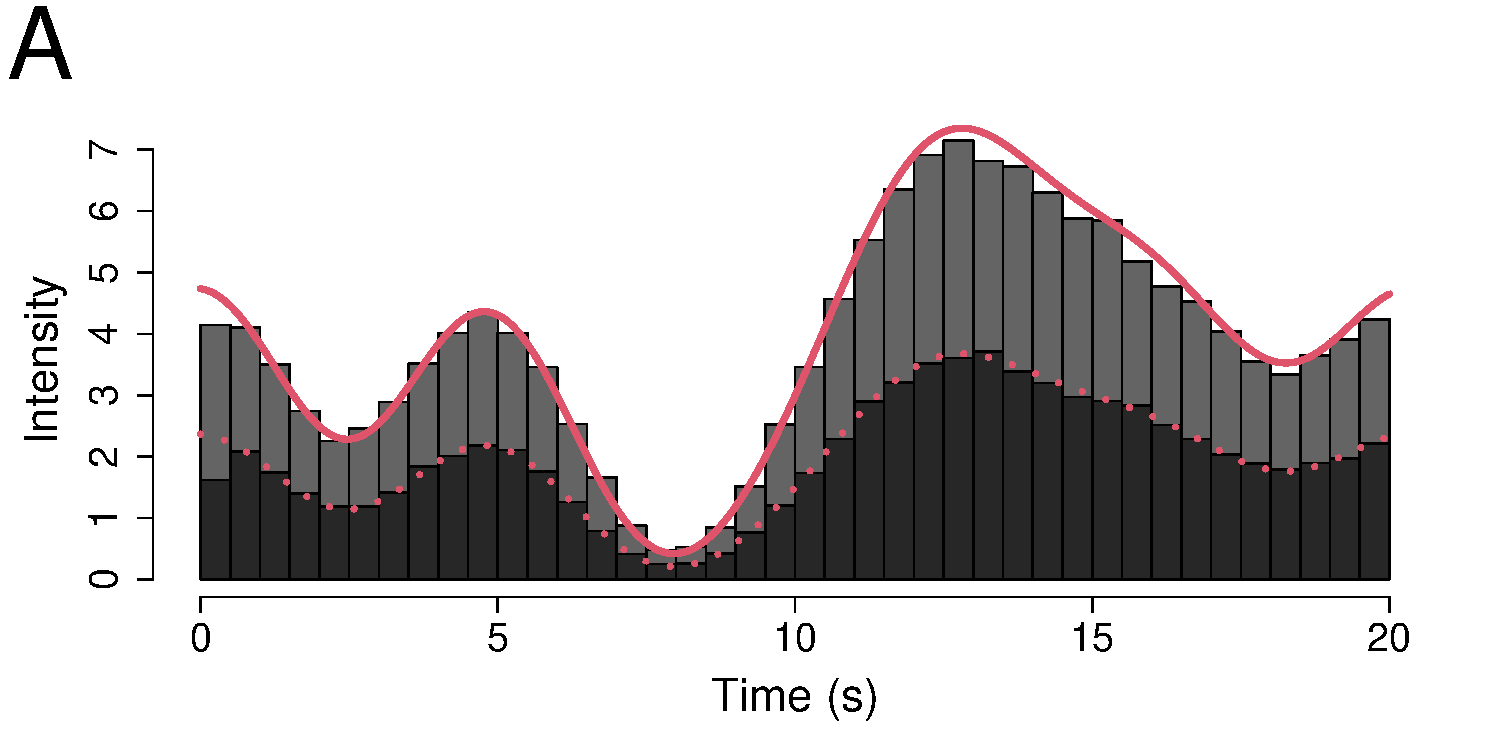
\includegraphics[width = 0.68\linewidth]{CompareHist}}
	\end{subfloat}
	\begin{subfloat}{
	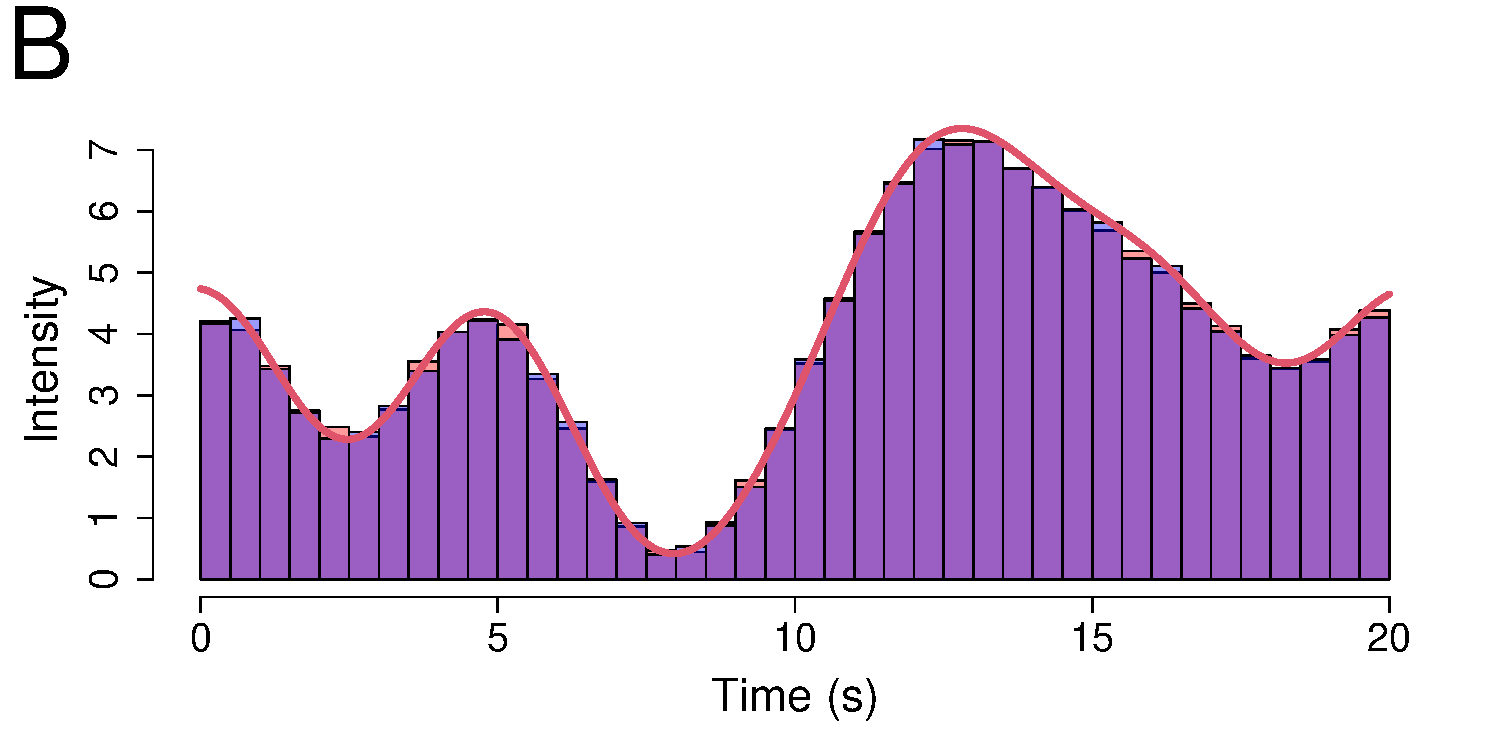
\includegraphics[width = 0.68\linewidth]{CompareHist_Dist}}
	\end{subfloat}	
		\caption{Comparing the intensity function --- the red line in both plots --- to histograms of 1000 simulated spike sequences. In (A) the light and dark boxes correspond to spikes generated from the model with Gamma ISI distributions with parameters Gamma(1.8,1.8) and Gamma(3.6,1.8) respectively. In (B) the spike sequences are simulated from a Gamma(1.8,1.8) and an Inverse Gaussian (1,1.8) resulting in the histograms in blue and red respectively, whose overlap is purple.  }
\label{fig:CompareHist}
\end{center}
\end{figure}


    
    
%Example to compare multi dists?
Moreover, by constraining the stationary distributions in this way we can directly compare intensity functions from models with different ISI distributions. For example we could compare the intensity function from a Gamma and Inverse Gaussian. If the intensities were similar this would show consistency between the models.   

To show this, consider a third model with the same intensity function but whose ISI distribution follows an Inverse Gaussian with parameters $\mu =1$ and $\lambda=1.8$, which has mean one. We simulate 1000 spike sequences from this model. In Figure \ref{fig:CompareHist}(B), we compare the mean spike rate of this model with the first model ---  Gamma ISI distribution with mean one. The red and blue boxes correspond to binning the spike sequences from the Inverse Gaussian and Gamma models respectively. The overlap of the boxes is coloured purple. We see that the mean spike rate from both models are near identical. This shows that the intensity function of both models correspond to the mean spike rate, thus allowing us to compare intensity functions from models using different underlying probability distributions. 

Note however, that even though the two models have the same intensity function this does not mean that the models are identical. The statistics of individual spike sequences could vary dramatically. For example, in Figure \ref{fig:Rasta} we show rastor plots of $20$ sequences corresponding to the Gamma and Inverse Gaussian models respectively, used in Figure \ref{fig:CompareHist}(B). We see that the spikes from the Inverse Gaussian model has more regular spikes than those from the Gamma model. 


%Furthermore, we can simulate 1000 spike sequences from the Inverse Gaussian ISI distribution with identical intensity function as above and parameters $(1.8,1)$, whose mean is one. In figure \ref{fig:CompareHist}(B) we compare the histograms of the simulated spike sequences from the Inverse Gaussian (red) and Gamma (blue) models, we see that the histograms are close to identical --- the overlap is coloured purple --- and the mean spike rate is the same for both models and equal to the intensity function. 

 %Figure ISI parameter
   \begin{figure}[t!]
   \begin{center} 
    \subfloat{{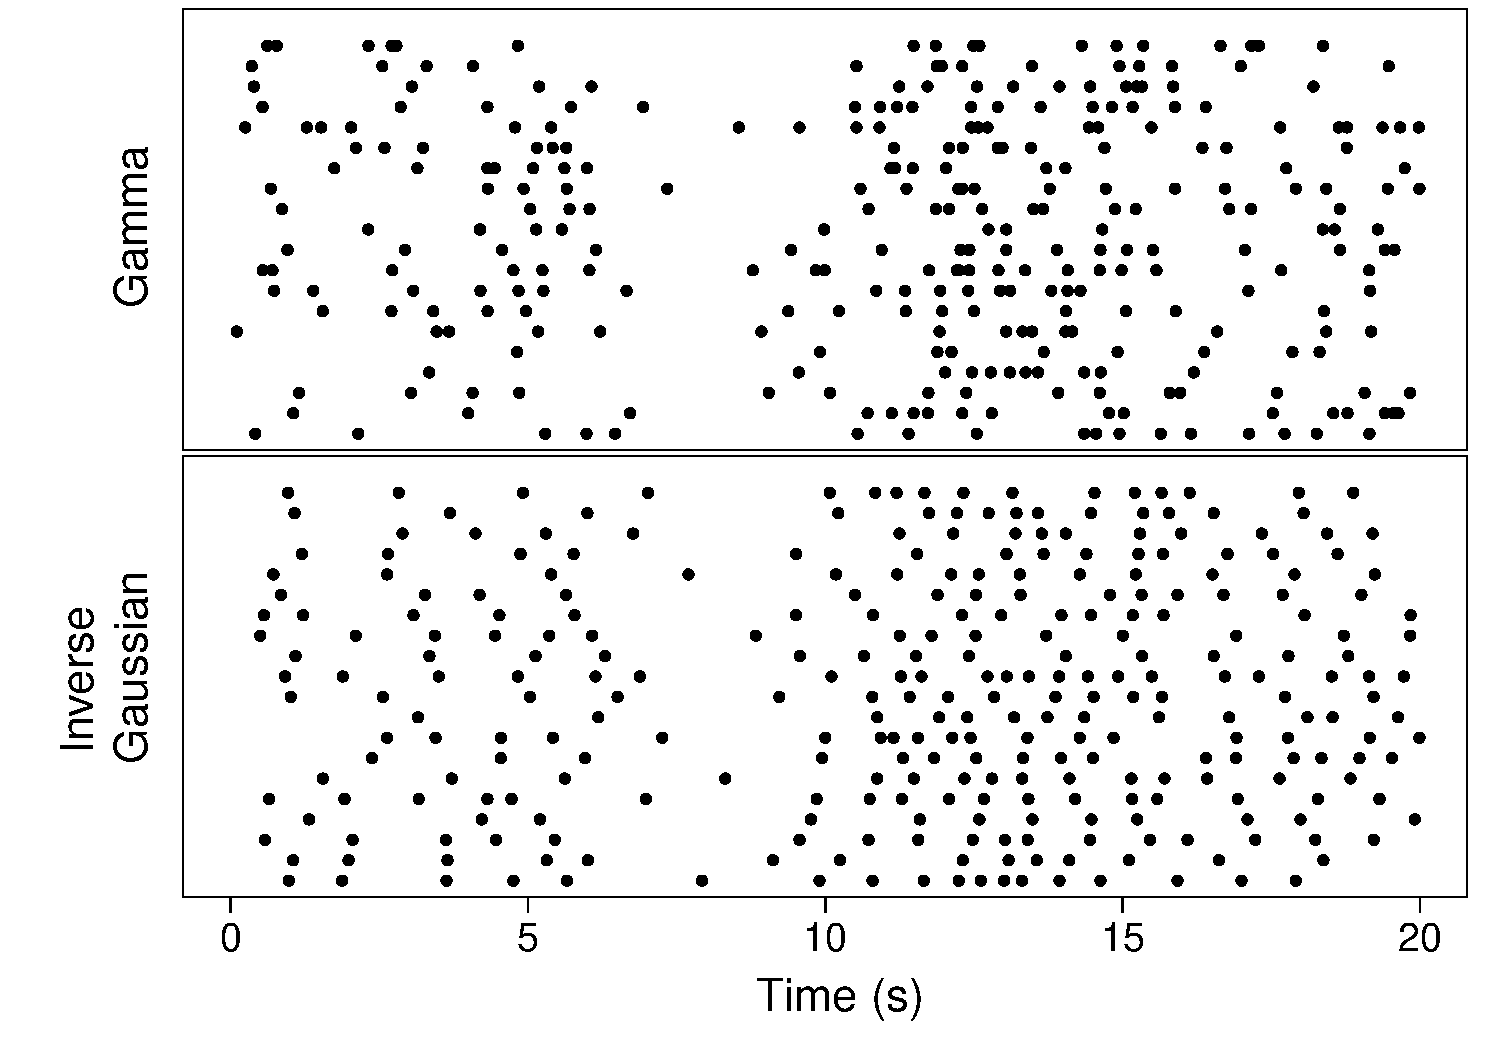
\includegraphics[width=0.8 \linewidth]{Image} }}    
    \caption{Rastor plots comparing $20$ spike sequences drawn from the models in Figure \ref{fig:CompareHist}(B). Both models share the same intensity function. The inhomogeneous Gamma has parameters $\alpha = 1.8$ and $\beta = 1.8$ and the inhomogeneous Inverse Gaussian has parameters $\mu=1$ and $\lambda = 5$.} 
      \label{fig:Rasta}
    \end{center} 
    \end{figure}
    
Applying the time-rescaling transformation to the new restricted one-parameter version of the stationary distributions leads to the following inhomogeneous ISI distributions: the Exponential ISI distribution
$$
 g_{\mathrm{EXP}}(t,s|x) = x(t) e^{-X(s,t)},
 $$

the Gamma ISI distribution
$$
 g_{\mathrm{GAM}}(t,s| x, \gamma) =  \frac{\gamma x(t)}{\Gamma ( \gamma )} \big[ \gamma X(s,t) \big]^{\gamma -1} \exp \left\{ - \gamma X(s,t)  \right\},
$$
 the Inverse Gaussian ISI distribution
 $$
  g_{\mathrm{IG}}(t,s| x,\lambda) =  x(t) \bigg( \frac{\lambda}{2\pi X(s,t)^3} \bigg)^{0.5} \exp \bigg\{-\frac{\lambda(X(s,t)-1)^2}{2 X(s,t)} \bigg\},
 $$
 
 the Log Normal ISI distribution
 $$
  g_{\mathrm{LN}}(t,s| x, \mu ) = \frac{x(t)}{2 X(s,t) \sqrt{\pi \mu}} \exp \left\{ -\frac{(\log X(s,t) + \mu)^2}{4\mu} \right\},
 $$
  
 and the Weibull ISI distribution
$$
 g_{\mathrm{W}}(t,s|x,k) = \frac{x(t)k}{\frac{1}{\Gamma(1+1/k)}} \left( \frac{X(s,t)}{\frac{1}{\Gamma(1+1/k)}} \right)^{k-1} \exp \left\{ -\left( \frac{X(s,t)}{\frac{1}{\Gamma(1+1/k)}} \right)^k \right\}.
 $$



 
 %Summary 
 Thus, we have created five inhomogeneous ISI distributions based on the Exponential, Gamma, Inverse Gaussian, Log Normal and Weibull probability distributions. The time-dependence of each distribution comes from the intensity function $x$ which represents the mean spiking rate. All the ISI distributions bar the Exponential also have a single ISI parameter $\gamma$, $\lambda$, $\mu$ and $k$ for the Gamma, Inverse Gaussian, Log Normal and Weibull respectively. This parameter describes the shape/variance of the ISI distribution. 
 
 We will use the five ISI distributions --- namely Exponential, Gamma, Inverse Gaussian, Log Normal and Weibull  --- in our analysis of \ce{Ca^2+} spike sequences and explore which, if any, of the distributions best describe \ce{Ca^2+} data and what we can learn from the results.

%Paragraph on how these compare to previous work. 
%So now that we have decided on the ISI distributions we are going to apply, how do they relate to previous work? 


We now compare our inhomogeneous ISI distributions with those used in Tilunaite et al \cite{AGNE:1}.
%\cite{AGNE:1}
 They used three ISI distributions in their work, the so-called inhomogeneous Poisson (IP), inhomogeneous Gamma (IG) and the inhomogeneous Inverse Gaussian (IIG). The IP and IG agree exactly with our Exponential ISI distribution and Gamma ISI distribution. However, their IIG ISI distribution has a different parameterisation to our Inverse Gaussian ISI distribution. Their model is generalised from the Inverse Gaussian with parameters $(1,\alpha)$ whereas our model is based on the parameters $(\lambda ,1)$. We do not use their parameterisation because the mean is not one, and as such the intensity function $x$ does not agree with the mean spiking rate. 

Thus the ISI distributions we consider builds upon previous work using the Exponential and Gamma ISI distributions and explores new distributions including the Log Normal and Weibull, which could better describe the \ce{Ca^2+} spike sequences. Moreover, we have constructed the models in such a way that the intensity function coincides with the mean spiking rate. This allows for easier interpretation of the model parameters.

%It is important to note that although we may find that one probability distribution best describes the \ce{Ca^2+} spikes, there may exist a better untested model. In particular, in the above example if we only tested the Exponential, Log Normal and Weibull distribution we would have said that the Weibull distribution is the best candidate to describe the \ce{Ca^2+} spikes. Thus, we have shown that the choice of ISI distribution is vital when considering stationary models. 

\bibliographystyle{unsrt}
\bibliography{bibliography} 

\end{document}